\documentclass{article}
%\usepackage{enumitem}
\usepackage{graphicx}
\graphicspath{ {./CS3_Assignment3/} }
\begin{document}
\title{Assignment 3}
\author{Brandon Kamplain and Mia Weber}

\maketitle
\newpage

\section{Question 1:}
Please see attached files. (main.cpp, Horspool.cpp, KMP.cpp, Karp-Rabin.cpp)

\section{Question 2:}

\begin{center}
\noindent Adjacency Matrix:

\begin{tabular}{c || c | c | c | c | c | c | c | c | c | c |} 
& 0 & 1 & 2 & 3 & 4 & 5 & 6 & 7 & 8 & 9 \\  [0.5ex] 
\hline\hline
0 & $\infty$ & 6 & 10 & $\infty$ & $\infty$ & $\infty$ & $\infty$ & $\infty$ & $\infty$ & $\infty$ \\ 
\hline
1 & 6 & $\infty$ & 12 & 11 & 14 & $\infty$ & $\infty$ & $\infty$ & $\infty$ & $\infty$ \\
\hline
2 & 10 & 12 & $\infty$ & 12 & $\infty$ & $\infty$ & 8 & 16 & $\infty$ & $\infty$ \\
\hline
3 & $\infty$ & 11 & 12 & $\infty$ & $\infty$ & 6 & 3 & $\infty$ & $\infty$ & $\infty$ \\
\hline
4 & $\infty$ & 14 & $\infty$ & $\infty$ & $\infty$ & 4 & $\infty$ & $\infty$ & 6 & $\infty$ \\ 
\hline
5 & $\infty$ & $\infty$ & $\infty$ & 6 & 4 & $\infty$ & $\infty$ & $\infty$ & 12 & $\infty$ \\ 
\hline
6 & $\infty$ & $\infty$ & 8 & 3 & $\infty$ & $\infty$ & $\infty$ & $\infty$ & 16 & 6 \\
\hline
7 & $\infty$ & $\infty$ & 16 & $\infty$ & $\infty$ & $\infty$ & $\infty$ & $\infty$ & $\infty$ & 8 \\
\hline
8 & $\infty$ & $\infty$ & $\infty$ & $\infty$ & 6 & 12 & 16 & $\infty$ & $\infty$ & 13 \\
\hline
9 & $\infty$ & $\infty$ & $\infty$ & $\infty$ & $\infty$ & $\infty$ & 6 & 8 & 13 & $\infty$ \\  [1ex] 
\hline
\end{tabular}
\end{center}

\noindent Using Prim.cpp we get the following edge list:

\begin{center}
\begin{tabular}{||c | c | c||} 
\hline
Edge & Weight & Total Cost \\ [0.5ex] 
\hline\hline
0 $\rightarrow$ 1 & 6 & 6 \\ 
\hline
0 $\rightarrow$ 2 & 10 & 16 \\
\hline
6 $\rightarrow$ 3 & 3 & 19 \\
\hline
5 $\rightarrow$ 4 & 4 & 23 \\
\hline
3 $\rightarrow$ 5 & 6 & 29 \\ 
\hline
2 $\rightarrow$ 6 & 8 & 37 \\ 
\hline
9 $\rightarrow$ 7 & 8 & 45 \\
\hline
4 $\rightarrow$ 8 & 6 & 51 \\
\hline
6 $\rightarrow$ 9 & 6 & 57 \\  [1ex] 
\hline
\end{tabular}
\end{center}

\noindent Using the following edge list generated from Prim.cpp we get the following minimal spanning tree:

\begin{center}
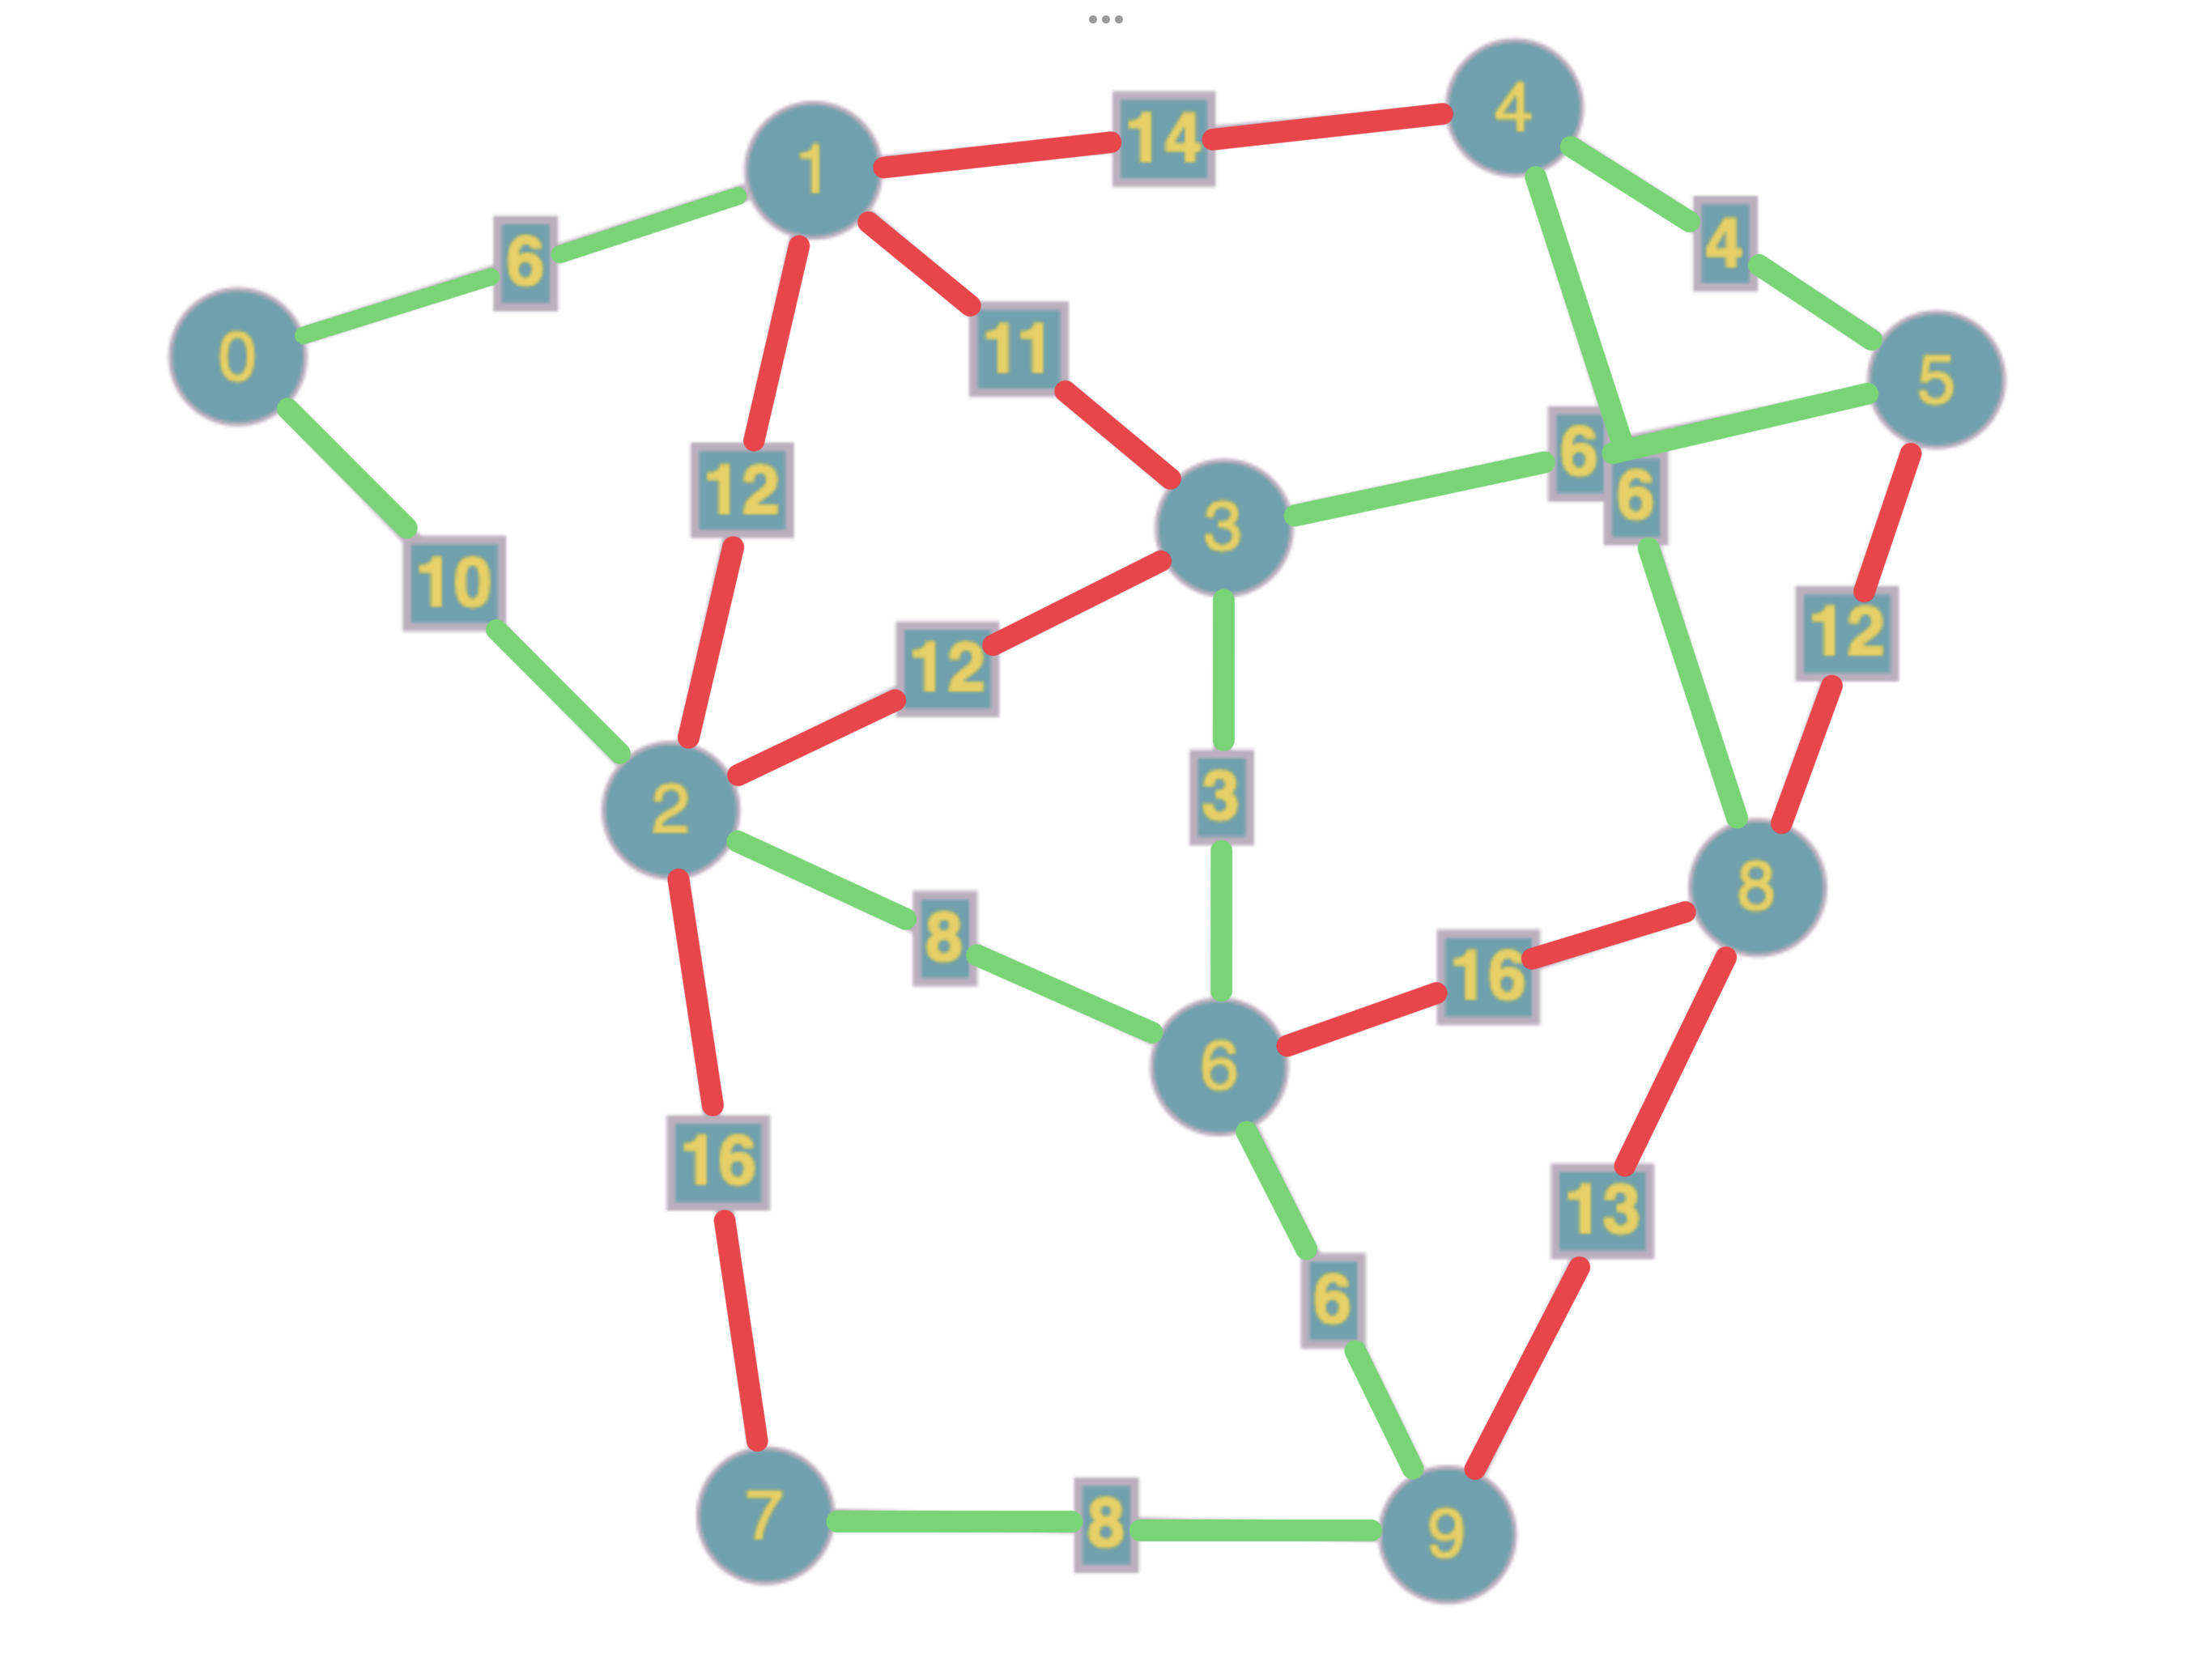
\includegraphics[width=\textwidth]{colorizedMST.jpeg}
\end{center}

\paragraph{\linebreak I declare that all material in this assessment task is my work except where there is clear acknowledgment or reference to the work of others. I further declare that I have complied and agreed to the CMU Academic Integrity Policy at the University website.
\linebreak  http://www.coloradomesa.edu/student-services/documents
\linebreak \linebreak Author’s Name: Mia Weber UID: 700510845 Date: 10/6/2022
\linebreak Author's Name: Brandon Kamplain UID: 700510289 Date: 10/6/2022}


\end{document}